\section{Studies with the Hadron Outer Calorimeter}
In the barrel region of the CMS experiment the hadronic calorimeter has a outer component placed just behind the solenoid and before the first muon stations (BILD). 
This subdetector is called the hadron outer (HO) calorimeter and is a tail catcher for jets leaking out of the inner hadronic calorimeter.
In this section first of all the HO system and its readout structure are introduced.
Then some studies on detection efficiency of muons using 2012 data are shown. The analysis of the detection efficiency for cosmic muons from GRIN data is conclusively dealt with.
	\subsection{The Hadron Outer (HO) Calorimeter}
		to do with Andreas
  		\subsubsection{Benefits and constraints}
			to do with Andreas
  		\subsubsection{Design of the system}
			to do with Andreas
	\subsection{Readout logic and DIGI structure}
		to do with Andreas
  		\subsubsection{Readout setup}
			to do with Andreas
	\subsection{Studies on detection efficiency of prompt muons using 2012 data}
		Due to the similarity of the setup of HO and MTT by studying the HO signals we expect to find answers to some open questions concerning the MTT concept like the muon detection capability of a
		scintillator system  read out by SiPMs e.g. Therefore the detection efficiency for tight ID muons from Run A of the 2012 data in HO has been studied.
		For this purpose the muons have to fulfill some selection createria and they have to be accepted by the HO system since HO has inefficient areas due to the supporting structures of CMS like the
		chimney (REF).
		\subsubsection{Muon selection and acceptance by HO}
		\label{thesectionhere}
			To be sure to have no fake muons going through the HO tiles some selection createria are set for the reconstructed muons.
			First of all only reco::muons which are also global muons are chosen.
			Then a cut on the pseudorapidity of the muons $|\eta_\mu| < 0.9$ is applied to be ensure that they are in the barrel region and especially in the region of HO.
			The muons also should have a tight ID.
			In (REF) all requirements on muons to be a tight muon are given.
			Essential for the tight ID definition is the consideration of good primary vertices.
			For this purpose a good vertex filter is applied:
			Using the vertex collection \textit{offlinePrimaryVertices} only vertices are chosen whose:
			\begin{itemize}
				\item minimum number of degrees of freedom is 4,
				\item maximum distance on the $z$ axis to the origin of the coordinate system is 24\,cm,
				\item maximum $d_0$ is 2\,cm.
			\end{itemize}
			Furthermore all these tight muons have to have an particle flow based combined relative isolation defined as
			\begin{equation}
				\frac{\sum{E_T^{chHad}} + \sum{E_T^{neutHad}} + \sum{E_T^\gamma}}{p_T}
			\end{equation}
			where $E_T^{chHad}$ is the transverse energy of a charged hadron in a cone of $dR = 0.4$ around the muon, $E_T^{neutHad}$ same for a neutral hadron and $E_T^\gamma$ for a photon.
			Since the HO system doesn't cover the whole $\eta$-$\phi$ plane - for example there are no tiles between the wheels - and also since the HO system has some areas with elecronic inefficiencies the
			cut on $|\eta_{mu}|$ mentioned before is not sufficient and a more sophisticated geometrical acceptance have to be requiered. 
			This is done using the \textit{MuonHOAcceptance} class implemented in the software framework of CMS.
			\textit{MuonHOAcceptance} knows the entire HO geometry and allows boolean decisions on whether a muon is in the geometrical acceptance of the HO or not and also whether a muon is in the acceptance region of
			tiles which are working properly.
			\begin{figure}[htbp]
				\centering
				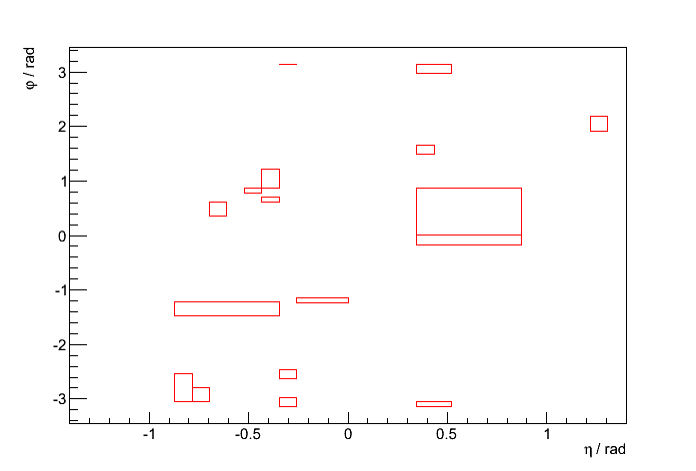
\includegraphics[width=0.45\textwidth]{Figures/erdogan/deadregions.png}
				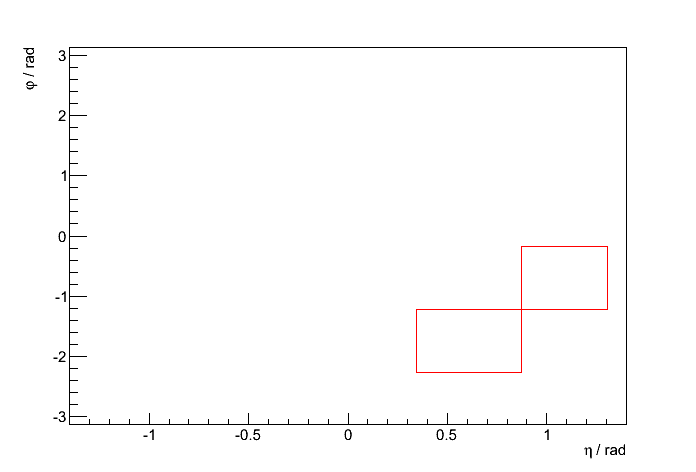
\includegraphics[width=0.45\textwidth]{Figures/erdogan/sipmregions.png}
				\caption{Left: In the $\eta-\phi$ plane, the red rectangles are showing the regions where HO is insensitive due to the supporting material or electrical issues. Right: In red rectangles the
				acceptance regions for tiles with SiPM readout.}
				\label{fig:ho_acceptance}
			\end{figure}
			It is also possible to accept or reject muons in regions with SiPM instrumented tiles (figure \ref{fig:ho_acceptance}).
			\begin{figure}[htbp]
				\centering
				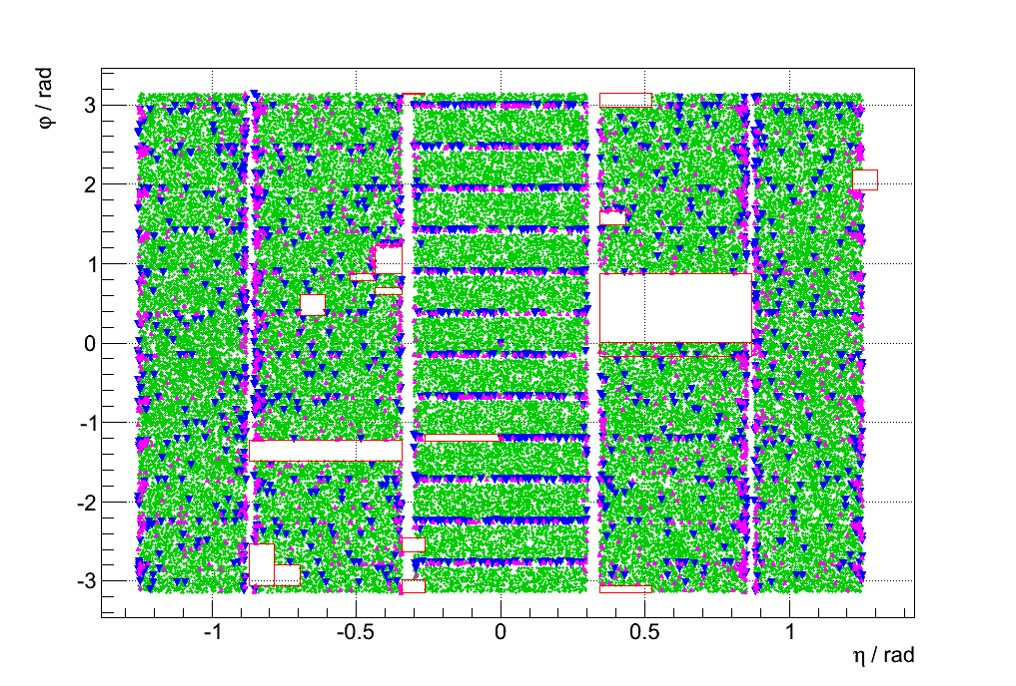
\includegraphics[width=0.45\textwidth]{Figures/erdogan/simhits_wo_deta_dphi.png}
				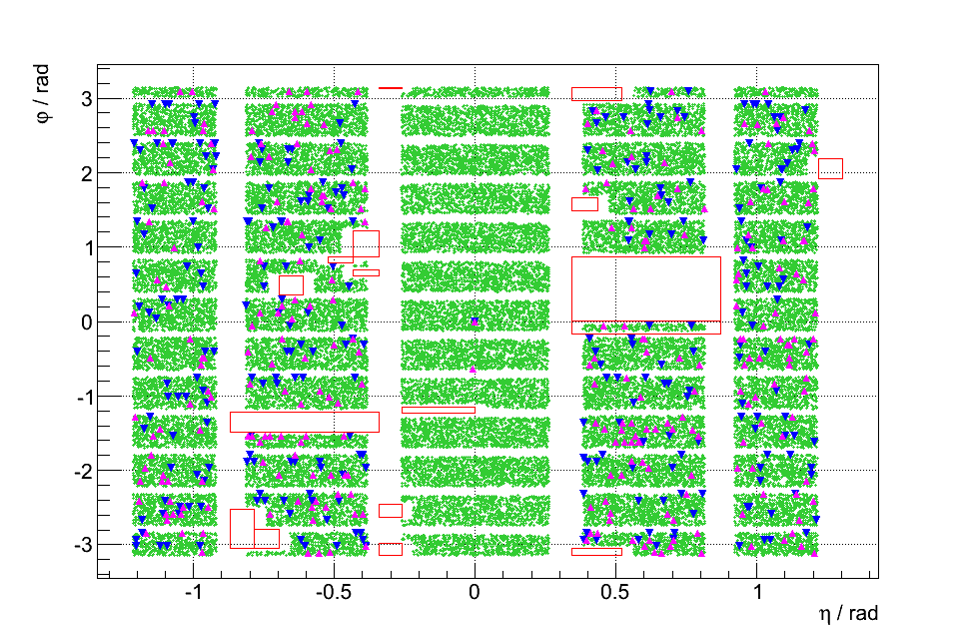
\includegraphics[width=0.45\textwidth]{Figures/erdogan/simhits_with_deta_dphi.png}
				\caption{Left: $\eta-\phi$ distribution of simulated hits of muons with $p_T = 100$\,GeV (muon gun). In green, hits from geometrically accepted muons with energy depositions above 1.4\,MeV, in
				blue, same for muons with energy depositions between 0 and 1.4\,GeV and in magenta, for muons with no energy deposition at all. The threshold at 1.4\,MeV is motivated by Bethe-Bloch formula, which
				predicts an energy deposition of > 1.4\,MeV for muons going through 1\,cm material (REF). Right: The same distribution with the safety distances $d\eta = 0.04$ and $d\phi = 0.017$ from the edges
				of the HO panels.}
				\label{fig:simhits_in_acceptance}
			\end{figure}
			In figure \ref{fig:simhits_in_acceptance} the $\eta-\phi$ distribution of simulated hits of muons with $p_T = 100$\,GeV (muon gun) in HO is shown.
			According to it a large fraction of the accepted muons deposit energies predicted by Bethe-Bloch (REF).
			But there are muons going through HO tiles but depositing very low energies or no energy at all.
			These muons are located particularly at the edges of the HO panels.
			Having only scratched the HO tiles barely, the transition is only enough for either very low depositions or nothing.
			Therefore it is helpful to reject those muons by defining safety distances from the edges of the panels as it is shown on the right hand side in figure
			\ref{fig:simhits_in_acceptance}.
			By having these safety distances there is only a very small fraction of muons depositing low energies with uniform $\eta-\phi$ distributions in the panels due to the insensitive areas between
			the tiles.
			With all these considerations 1.139.214 muons could be selected in Run A of 2012 data taking (CutFlow).
		\subsubsection{Matching of the muons to the corresponding HO tiles}
			Being selected as in \ref{thesectionhere} described the muons now have to be matched to the correct HO tiles.
			This is done by using the standard tracking tool \textit{TrackDetMatchInfo}.
			Doing a helix approximation this tool collects the information along a track.
			Among this information also HO related parts like the detector IDs of the tiles crossed by the muon, the reconstructed hits in these tiles or the global position of the track at HO etc. can be
			found.
			If one of the IDs of the HO tiles crossed by a muon is the same as one of the IDs of a reconstructed hit in the HO system, then this muon is matched to that tile.
			Since no additional requirements like to have a certain energy e.g. on the reconstructed hits are done, this procedure is a very loose one.
		\subsubsection{Detection efficiency for prompt muons}
			Even with the loose procedure of matching muons to the correct tiles only 694.920 muons could be matched to the HO tiles with a reconstructed hit in it. This leads to an efficiency of $61\,\%$.
			This very low ration of matched muons to all selected muons is dominated by the noise behaviour of the HPDs as decribed in (REF).
			Looking into the SiPM tiles only one expect a higher efficiency due to the better S/N ratio of the SiPMs compared to the HPDs.
			But also here out of selected 79.745 muons only 44.682 muons can be matched which means an efficiency of $56\,\%$.
			The reason for that very low efficiency is a known problem with the slow control of the first generation SiPMs used for the readout of $7\%$ of the HO tiles during 2012 data taking.    
	\subsection{Studies on detection efficiency of cosmic muons using the GRIN data} 
		In November 2013 for one week CMS has taken data of cosmic muons during a global run (GRIN = \textbf{G}lobal \textbf{R}un \textbf{I}n \textbf{N}ovember).
		For this operation the magnet was switched off.
		The aim was to check the functionality of subsystems after the long operation break due to the long shutdown 1.
		However the data can also be used to study the response behaviour of different upgraded subsystems, like HO.
		\subsubsection{Detector setup and preperation of the data}
			This HO system was partially in use during GRIN and the following parts were instrumented with the next generation SiPMs:
			\begin{itemize}
				\item All YB-2, YB-1,
				\item 7 of 12 sectors in YB0 (1,4,5,7,8,9,12),
				\item 2 of 12 sectors in YB+1 (3,4),
				\item 2 of 12 sectors in YB+2 (3,4)
			\end{itemize}
			These SiPMs have a better functionality compared to the first generation SiPMs used during the first run.
			Since the cosmic trigger was given by the moun system in the wheels YB+1, YB+2 and YB0 only the data from the corresponding parts of HO can be analyzed.
			Additionally only a few runs are marked as good for HCal/HO.
			These are 216232, 216311, 216312, 216420, 216423 and 216450.
			Having considered that the RAW data of muons has to be reconstructed according to the standard cosmic reconstruction procedure of CMS.
			In this note we won't decribe in detail the reconstruction of the hits in the HO system, since the study in this section is concentrated on the DIGI information of HO.
		\subsubsection{HO DIGI information}
			The CMS data format DIGI contains the information of the detector response to a physical process like a muon transition.
			In case of HO the measured signal is stored as counts of an analog-to-digital-converter (adc) for 10 timeslices in a HO DIGI.
			Each timeslice takes 25\,ns.
			For the calibration of the HO DIGIs it is possible to use several records registered during the data taking, like the HCalPedestalRecord or HCalElectronicsRecord.
			A text calibration can be alternatively done using text files filled with calibration values determined by hand.
			For this study such a text calibration is done setting all pedestal corrections to 0, all gain corrections to 1 and all slope corrections to 1.
			This ensures the studied signal to be unbiased by the calibration itself, since for such short runs like GRIN the calibration by records are not so expressive.
			In figure (\ref{fig:adc_vs_ts}) the calibrated adc counts versus the timeslices in which they are measured are shown.
			\begin{figure}[htbp]
				\centering
				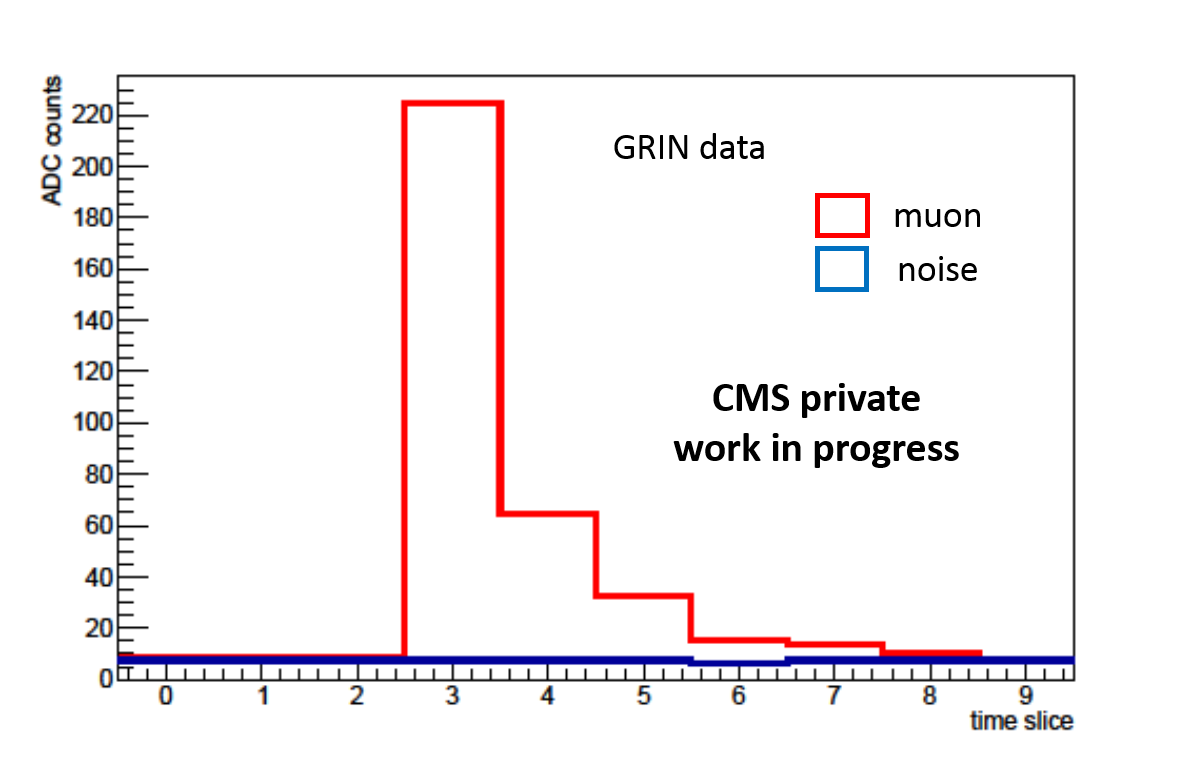
\includegraphics[width=0.45\textwidth]{Figures/erdogan/adc_vs_ts.png}
				\caption{The calibrated adc counts versus the timeslices in which they are measured: In blue a tile is chosen, where no muon is gone through (noise). In red is a tile with muon transition shown.}
				\label{fig:adc_vs_ts}
			\end{figure}
			In case of muon transition the measured adc counts in the corresponding timeslices are clearly higher then without muon transition.
			This means that distinguishing muon signal from noise should be possible.
		\subsubsection{Purity studies}
			In section (REF) the funtionality of SiPMs is already discussed.
			There the meaning of a finger spectrum as the signal of a SiPM is also described.
			Now concerning the HO data from GRIN such a spectrum can be studied.
			Therefore the signal in one randomly chosen HO tile is considered.
			In figure (\ref{fig:noise_low}) this signal distribution as a function of adc counts is shown for the tile XY.
			\begin{figure}[htbp]
				\centering
				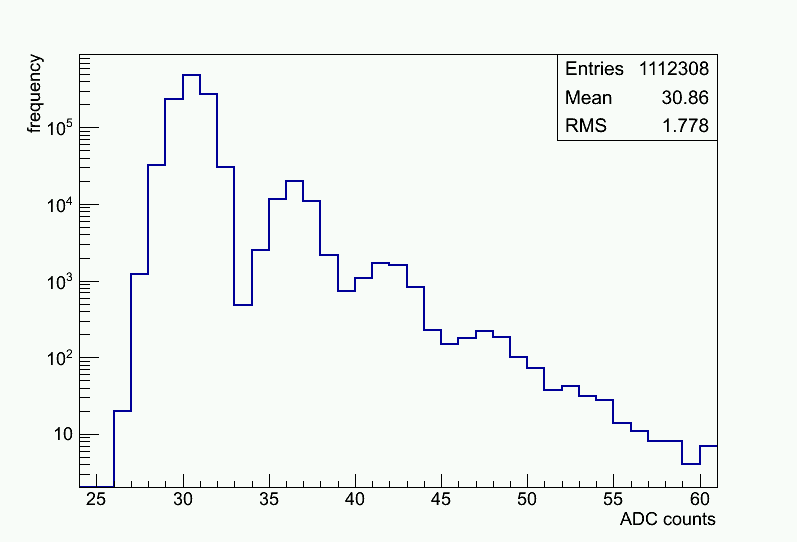
\includegraphics[width=0.45\textwidth]{Figures/erdogan/noise_low.png}
				\caption{The signal distribution as a function of adc counts for the tile XY.}
				\label{fig:noise_low}
			\end{figure}
			The first peak is the pedestal of the signal being at 36 adc counts.
			Furthermore there are 3 additional peaks corresponding to the up to 3 firing pixels of the SiPM.
			The distance between the peaks, which is the gain of the SiPM, is at 6 adc counts.
			All these observations are consistent with the expectations from the HO detector performance group (REF to ANDREAS).
			Since this study is done with only one tile per event the statistic is relatively low.
			To get more statistic and study the behaviour of the noise distribution with this higher statistic all tiles per event without a muon transition are considered (figure (REF)).
			To do this first of all the tile where the muon went through has to be traced.
			This is done by the TrackDetMatchInfo tool described in subsection (REF).
			Afterwards a safety region of 3x3 tiles around this traced tile is defined.
			Now with all remaining tiles in all events the noise distribution can be considered (figure \ref{fig:noise_high}).
			\begin{figure}[htbp]
				\centering
				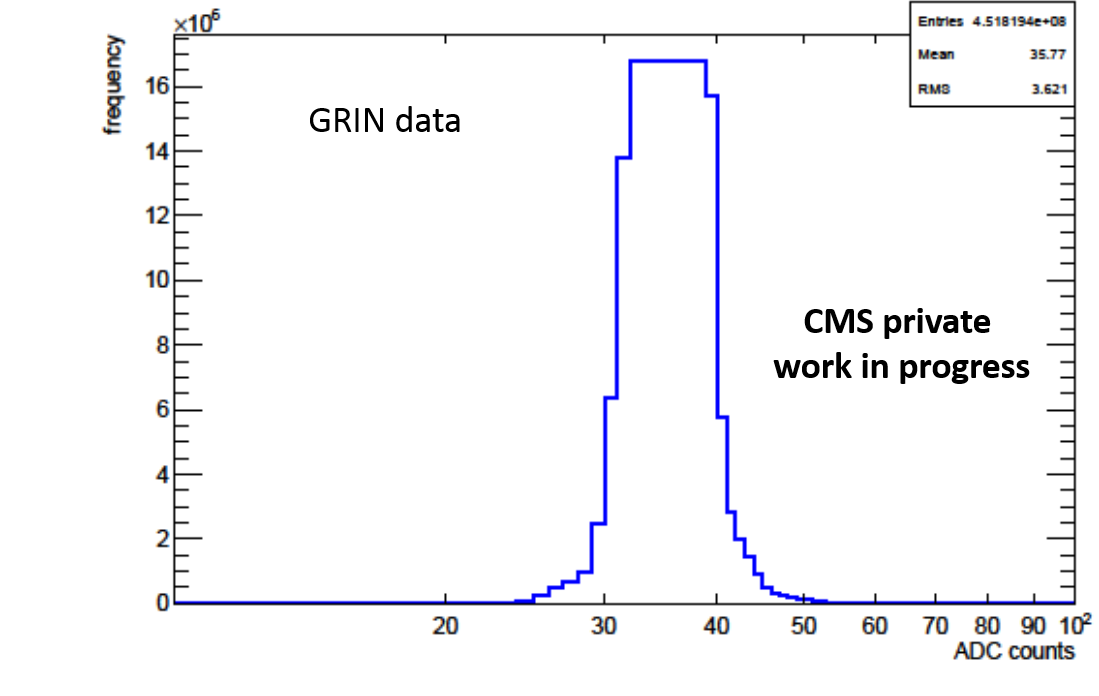
\includegraphics[width=0.45\textwidth]{Figures/erdogan/noise_high.png}
				\caption{The signal distribution as a function of adc counts for all tiles without muon transition.}
				\label{fig:noise_high}
			\end{figure}
			The mean is at 36 adc counts as expected and seen as pedestal in the distribution with low statistics (finger spectrum).
			Also the fingers are not visible anymore.
			The reason for this is the smearing of the finger due to their statistical uncertainty.
			Furthermore the distribution drops steaply in the higher bins until there is no significant signal anymore.
			It is therefore above 80 adc counts not expected the noise contribution in the signal to be significant.
			With this a purity definition of the muon signal can be done.
			In the section \ref{working_point} this value can be improved comparing the efficiency and the purity.
		\subsubsection{Efficiency studies}
			After having a method to estimate the purity the muon signal has to be analyzed.
			Using the TrackDetMatchInfo tool one can find the tiles where the muons are going through.
			Once the correct tiles are traced, the DIGI information can be looked into.
			For this purpose an integration over 4 timeslices is done to define the signal.
			The choice of the correct 4 timeslices is important and is done as described following:
			\begin{itemize}
			  \item Find the timeslice $i$ with the highest adc counts.
			  \item If $i$ between 1. and 7. timeslice (inclusively) add adc counts of timeslice $i-1$, $i+1$ and $i+2$ to the adc counts of $i$.
			  \item If $i=0$, $i=8$ or $i=9$ take timeslices 2,3,4 and 5 for the integration.
			\end{itemize}
			In figure (REF) the integrated value of adc counts is 
		\subsubsection{Working point for triggering muons}
		\label{working_point}
			todo
